% VisaAssist AI -- CMPE 491/492 Senior Design Project report
% Compile on Overleaf with: Compiler = pdfLaTeX, bibliography tool = Biber (Menu > Settings).
% Citation style: Chicago author-date (course requirement), via biblatex-chicago.
% When the department's official "Senior Design Project Final Report" template is
% published, move the chapters/ files into it; the chapter files do not depend on this preamble.

\documentclass[12pt,a4paper,oneside]{report}

% ---------------------------------------------------------------- fonts and language
\usepackage[T1]{fontenc}
\usepackage[utf8]{inputenc}
\usepackage{lmodern}
\usepackage[english]{babel}
\usepackage{csquotes}
\usepackage{microtype}

% ---------------------------------------------------------------- page layout
\usepackage[a4paper,top=2.5cm,bottom=2.5cm,left=3cm,right=2.5cm]{geometry} % 3 cm left margin for binding
\usepackage{setspace}
\onehalfspacing
\usepackage{fancyhdr}
\pagestyle{fancy}
\fancyhf{}
\fancyhead[R]{\small\nouppercase{\leftmark}}
\fancyfoot[C]{\thepage}
\renewcommand{\headrulewidth}{0.4pt}
\fancypagestyle{plain}{\fancyhf{}\fancyfoot[C]{\thepage}\renewcommand{\headrulewidth}{0pt}}

% ---------------------------------------------------------------- figures, tables, lists
\usepackage{graphicx}
\graphicspath{{figures/}}
\usepackage{booktabs}
\usepackage{tabularx}
\usepackage{longtable}
\usepackage[font=small,labelfont=bf]{caption}
\usepackage{enumitem}
\setlist{itemsep=2pt,topsep=4pt}
\usepackage[table]{xcolor}
\usepackage{listings}
\lstset{basicstyle=\ttfamily\footnotesize,breaklines=true,frame=single,columns=fullflexible}
\usepackage[nottoc]{tocbibind}

% ---------------------------------------------------------------- bibliography (Chicago author-date)
\usepackage[authordate,backend=biber,noibid]{biblatex-chicago}
\addbibresource{references.bib}

% ---------------------------------------------------------------- links (load late)
\usepackage[hidelinks]{hyperref}
\usepackage{bookmark}

% ---------------------------------------------------------------- project macros
\newcommand{\project}{VisaAssist AI}
\newcommand{\reqid}[1]{\texttt{#1}}          % requirement and rule identifiers, e.g. \reqid{FR-09}
\newcommand{\todo}[1]{\textcolor{orange!80!black}{[TODO: #1]}} % remove before submission
\newcommand{\semester}{Fall 2026}

\begin{document}

% ================================================================ front matter
\pagenumbering{roman}
% Title page. Check the department template for the exact layout before submission.
\begin{titlepage}
  \centering
  {\large ISTANBUL BILGI UNIVERSITY\par}
  {\large FACULTY OF ENGINEERING AND NATURAL SCIENCES\par}
  {\large DEPARTMENT OF COMPUTER ENGINEERING\par}
  \vspace{2.5cm}
  {\Large CMPE 491 -- Senior Design Project I\par}
  \vspace{1.5cm}
  {\huge\bfseries VisaAssist AI\par}
  \vspace{0.4cm}
  {\Large A source-grounded assistant and document pre-check\\for visa applications\par}
  \vspace{2.5cm}
  {\large Furkan Özdemir\par}
  {\large Student number: 123200171\par}
  \vspace{1.5cm}
  {\large Advisor: Doğan Çörüş\par}
  \vfill
  {\large \semester\par}
\end{titlepage}

\chapter*{Declaration}
\addcontentsline{toc}{chapter}{Declaration}
I declare that this report is my own work, that all sources used are cited, and that it has not
been submitted for any other course or degree. Tools used in the project, including AI
assistants for coding and writing support, are described in Section~\ref{sec:tools}.

\vspace{2cm}
\noindent Furkan Özdemir \hfill Date: \underline{\hspace{4cm}}

\noindent Signature: \underline{\hspace{5cm}}

\chapter*{Abstract}
\addcontentsline{toc}{chapter}{Abstract}
% 150--250 words. Write last. Structure: problem -- approach -- what was built -- how it is
% evaluated -- main result (fall: prototype; spring: measured comparison).
\todo{Problem: applicants in Türkiye prepare Schengen visa files from scattered official pages
and often submit incomplete or inconsistent documents.}
\todo{Approach: personalised checklists built from versioned official sources; rule-based
checks of the applicant's documents against the requirements and against each other; every
finding cites its source.}
\todo{Fall result: working prototype for the Netherlands (and the Norway translation rule),
employed and student profiles.}
\todo{Spring: hybrid (VLM + rules) vs LLM-only comparison on a labelled synthetic dataset.}

\noindent\textbf{Keywords:} visa application, document verification, rule engine,
retrieval-augmented generation, source monitoring

\chapter*{Özet}
\addcontentsline{toc}{chapter}{Özet}
% Turkish abstract, if the department template asks for one; otherwise delete this file and its \input.
\todo{Abstract'ın Türkçe karşılığı.}

\noindent\textbf{Anahtar kelimeler:} vize başvurusu, belge doğrulama, kural motoru,
kaynak destekli üretim, kaynak takibi


\tableofcontents
\listoffigures
\listoftables
\chapter*{Abbreviations}
\addcontentsline{toc}{chapter}{Abbreviations}
\begin{tabular}{@{}ll@{}}
  ADR  & Architecture Decision Record \\
  API  & Application Programming Interface \\
  CI   & Continuous Integration \\
  EU   & European Union \\
  FR / NFR & Functional / Non-functional Requirement \\
  KVKK & Turkish Personal Data Protection Law (Kişisel Verilerin Korunması Kanunu) \\
  LLM  & Large Language Model \\
  OCR  & Optical Character Recognition \\
  RAG  & Retrieval-Augmented Generation \\
  SGK  & Social Security Institution of Türkiye (Sosyal Güvenlik Kurumu) \\
  VLM  & Vision-Language Model \\
  YÖK  & Council of Higher Education of Türkiye (Yükseköğretim Kurulu) \\
\end{tabular}


% ================================================================ main matter
\clearpage
\pagenumbering{arabic}
\chapter{Introduction}\label{ch:intro}

\section{Problem and motivation}
% Why visa preparation is hard: scattered official pages, national differences, documents that
% must agree with each other, requirements that change. Who suffers (applicants without an agency).
\todo{2--3 paragraphs. Use the national differences in Table~\ref{tab:nl-no} as the concrete example.}

\section{Objectives}
The project pursues the five objectives of the approved proposal:
\begin{description}
  \item[H1 Personalisation] a checklist for the applicant's destination, visa type, profile and dates;
  \item[H2 Document pre-check] missing, outdated and mutually inconsistent documents are found before submission;
  \item[H3 Up-to-date information] changes of official sources are detected and reviewed;
  \item[H4 Source-grounded information] every requirement, finding and answer cites an official source;
  \item[H5 Measurable AI performance] the AI components are evaluated against baselines.
\end{description}

\section{Research questions}\label{sec:rq}
\begin{description}
  \item[AS1] Does a hybrid approach (vision-language model and rule engine) detect missing and
    inconsistent documents in multi-document application files better than an LLM-only approach,
    per error type (precision, recall, F1)?
  \item[AS2] How does the hybrid system compare with human reviewers in accuracy and time?
  \item[AS3] How accurately does source monitoring separate meaningful requirement changes from
    cosmetic page changes?
\end{description}

\section{Scope}
% ADR 0001 and its amendment.
The pilot covers the Schengen short-stay visa (type C) for tourism, applied for in Türkiye, for
employed and student applicants. The Netherlands is the main destination; Norway is added as a
second national layer because its checklist states a translation requirement. Predicting visa
decisions, legal advice and submitting applications on the applicant's behalf are out of scope.

\section{Contributions}
\todo{What is new compared with Chapter~\ref{ch:background}: versioned source-linked rules;
change detection that reaches only affected applicants; measured comparison with LLM-only and
human reviewers. See docs/positioning.md.}

\section{Organisation of the report}
\todo{One sentence per chapter.}

\chapter{Background and Related Work}\label{ch:background}
% Lecture 3: the review is the background of the research questions, not a list of papers.
% Each section ends with what is missing for this project.

\section{The Schengen short-stay visa in Türkiye}
The supporting documents for applicants in Türkiye are harmonised by the European Commission
\autocite{eu2021harmonised}; each member state adds national requirements, for example the
Netherlands \autocite{nl2025checklist} and Norway \autocite{no2025checklist}.

\begin{table}[ht]
  \centering
  \caption{National differences on top of the EU baseline (sources reviewed on 23 October 2026).}
  \label{tab:nl-no}
  \begin{tabularx}{\textwidth}{@{}lXX@{}}
    \toprule
    Topic & Netherlands & Norway \\
    \midrule
    Translation & not required & all documents in English or Norwegian \\
    General document age & not stated (photo $\leq$ 6 months) & no document older than 6 months \\
    Passport validity & 3 months after leaving the Schengen area & 3 months beyond the intended stay \\
    Financial means & bank statements of 3 months or proof of income & salary slips and bank movements of 3 months \\
    \bottomrule
  \end{tabularx}
\end{table}

\section{Document understanding and information extraction}
\todo{Survey-level overview \autocite{ding2026mllm,cui2021documentai}; what is measured
(single-document field extraction) and what is not (multi-document files).}

\section{Consistency checking across documents}
\todo{Closest work: DocChecker \autocite{chen2026contradictions}; limits of multimodal LLMs in
finding inconsistencies \autocite{selch2025prismm}; name matching \autocite{christen2006names}.
State the difference: external, versioned requirements plus document-to-document rules.}

\section{Retrieval-augmented generation and citation}
\todo{\textcite{gao2024ragsurvey}; citation quality \autocite{gao2023alce}; hallucination
\autocite{ji2023hallucination}.}

\section{Change detection of web pages}
\todo{\textcite{mallawaarachchi2020change}; semantic vs textual change \autocite{zhang2004xml}.}

\section{Similar systems}
\todo{Table from docs/related-work.md: open-source visa assistants and change monitors; none
reports measured accuracy.}

\section{Research gap}
\todo{3--4 sentences leading to AS1--AS3.}

\chapter{Requirements}\label{ch:requirements}
% Source: docs/requirements.md (v0.2). Keep IDs identical so tests and report agree.

\section{Stakeholders}
\todo{Applicant, administrator, researcher, advisor; table from requirements.md §2.}

\section{Functional requirements}
\todo{Table FR-01 -- FR-22 with goal, priority, semester (longtable).}

\section{Non-functional requirements}
\todo{NFR-01 -- NFR-10; privacy (KVKK) and languages (TR/EN) in detail.}

\section{Constraints}
One developer at about 15 hours per week over two semesters; an API budget of at most USD 20 per
month; evaluation on synthetic documents only.

\section{Success criteria}
Agreed with the advisor on 23 October 2026: every result is a comparison against a reference or
an alternative, never an isolated score.
\todo{Fall and spring criteria from requirements.md §6.}

\chapter{System Design}\label{ch:design}

\section{Architecture}
% ADR 0002: what runs in fall, what is deferred to spring and why.
\todo{Component diagram: web client, FastAPI, PostgreSQL with pgvector, source snapshots;
spring: job queue, AI service.}

\section{Requirement data and rule schema}
Requirements are data, not code. A destination's rule set is the EU baseline plus one national
layer; every checklist item and rule cites a source passage, and the loader rejects files whose
sources, documents, fields or field types do not match.
\todo{Rule kinds table (data/requirements/README.md) and one YAML example in a listing.}

\section{Data model}
\todo{ER diagram exported from docs/design/data-model.md; principle: YAML is the source of truth,
the database keeps versioned copies so every finding can be explained later.}

\section{Source monitoring}
\todo{Snapshot pipeline, manifest, administrator approval, notification of affected files only.}

\section{User interface}
The interface is one responsive web application with Turkish and English text
(Figure~\ref{fig:ui-checklist}; all screens in Appendix~\ref{app:screens}).
\begin{figure}[ht]
  \centering
  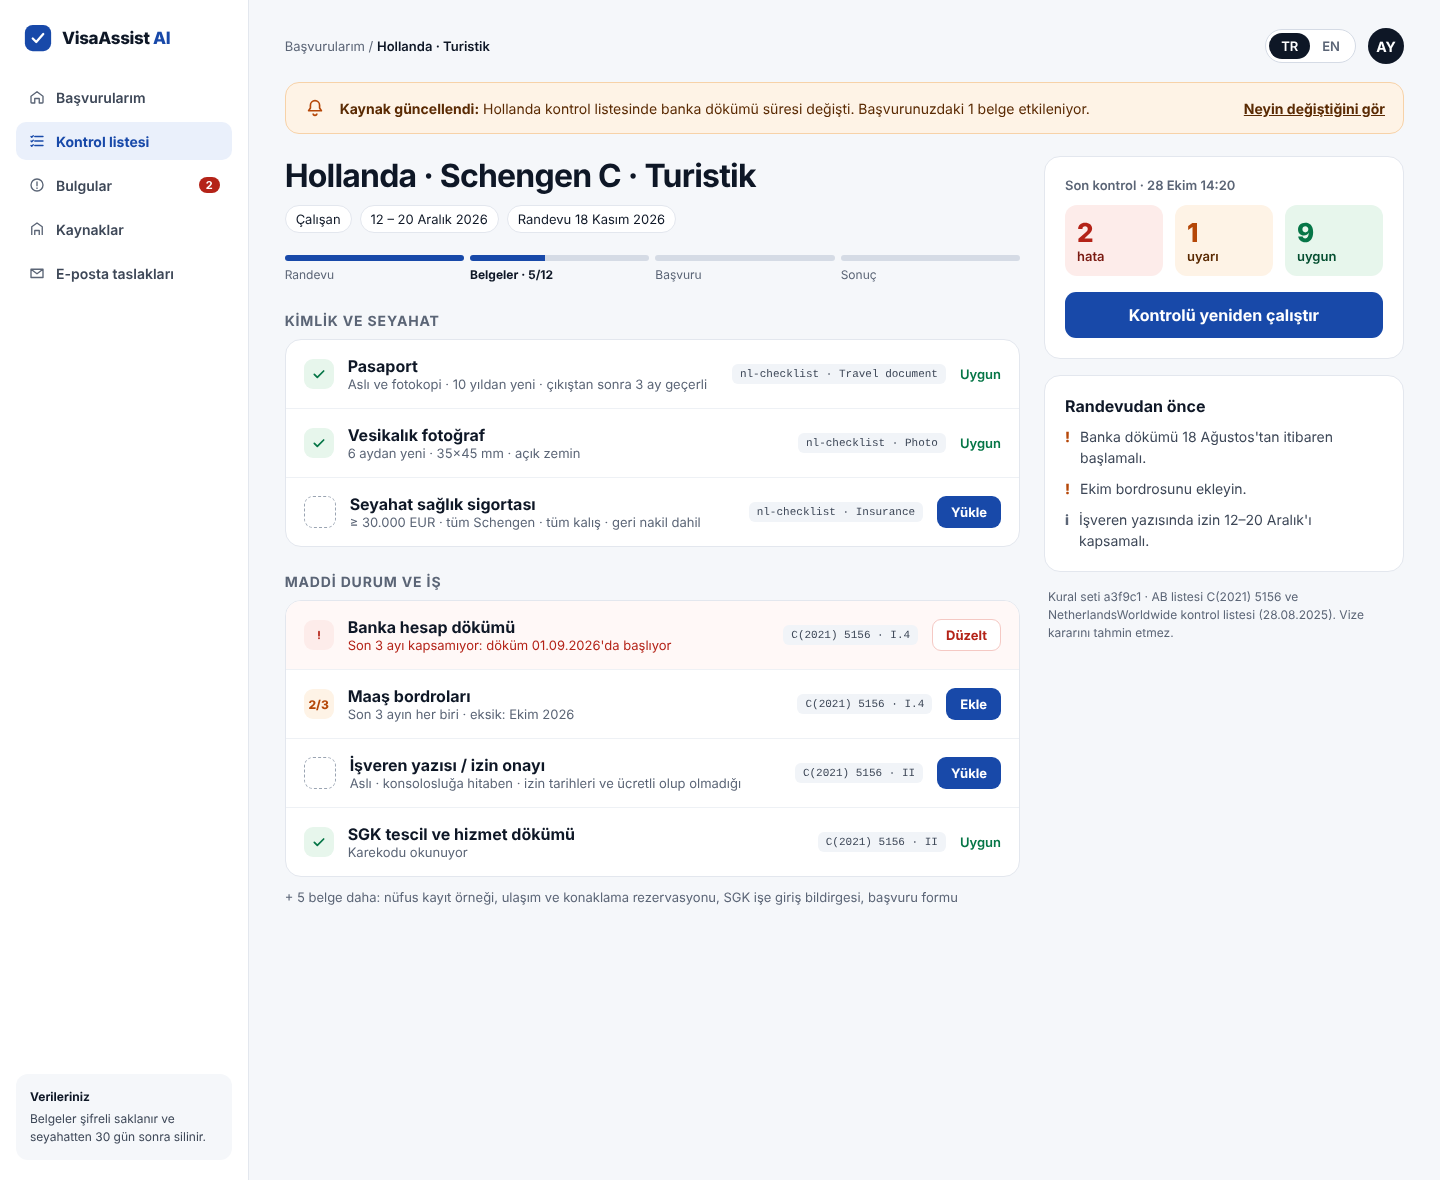
\includegraphics[width=\textwidth]{02-web-checklist.png}
  \caption{Application checklist: status, source tag and one action per document.}
  \label{fig:ui-checklist}
\end{figure}

\section{AI components and cost (spring)}
\todo{ADR 0003: model per task, four-layer cost control, estimates checked against measurement.}

\chapter{Implementation}\label{ch:implementation}
% Fall: what was built, with the key design choices and short code excerpts. Spring adds the AI parts.

\section{Development environment and tools}\label{sec:tools}
\todo{Python 3.12, FastAPI, SQLAlchemy, PostgreSQL 17 + pgvector, Docker Compose, uv, ruff,
pytest, GitHub Actions; AI assistants used for coding and writing support, with the developer
reviewing and committing every change.}

\section{Backend}
\todo{Health and readiness endpoints, settings, database access.}

\section{Requirement data and source snapshots}
\todo{Loader and cross-checks; snapshot command and manifest.}

\section{Rule engine}
\todo{W12: how a check kind is evaluated; reference date; findings with evidence.}

\section{Web client}
\todo{W10--W11.}

\chapter{Testing and Evaluation}\label{ch:evaluation}

\section{Test strategy}
\todo{Unit tests per rule, data-consistency tests, integration tests against PostgreSQL in CI;
branch protection requires a green run.}

\section{Fall evaluation}
\todo{Against the fall success criteria: generated vs hand-compiled checklist; findings vs
injected errors on demo files; checklist vs a general chat assistant's answer.}

\section{Spring experiment design}
\todo{Synthetic dataset and frozen test set; hybrid vs LLM-only (AS1); human reviewers (AS2);
labelled page versions with a text-diff baseline (AS3); metrics and reporting of model versions.}

\chapter{Project Management}\label{ch:management}

\section{Methodology}
Weekly increments, each an issue, a pull request with tests and a green CI run; decisions are
recorded as architecture decision records; the advisor is met every Friday.

\section{Schedule}
\todo{Work packages WP1--WP12 against weeks (ROADMAP.md); planned vs actual.}

\section{Risks}
\todo{Source changes, API cost, OCR quality, time; mitigation for each.}

\chapter{Ethics, Privacy and Legal Considerations}\label{ch:ethics}
\todo{KVKK: consent, encryption, retention, deletion, masking before external AI calls; synthetic
data only; the system does not predict or guarantee visa decisions; reuse of third-party code
and licences; accessibility.}

\chapter{Conclusion and Future Work}\label{ch:conclusion}
\todo{Fall: what the prototype does and how far the success criteria were met.
Spring: the remaining work packages and the experiments of Chapter~\ref{ch:evaluation}.}


% ================================================================ back matter
\printbibliography[heading=bibintoc,title={References}]

\appendix
\chapter{Rules of the Pilot}\label{app:rules}
\todo{Table of all rules (ID, check, source, severity), generated from data/requirements/ so the
report and the data cannot diverge.}

\chapter{User Interface Screens}\label{app:screens}

\begin{figure}[p]
  \centering
  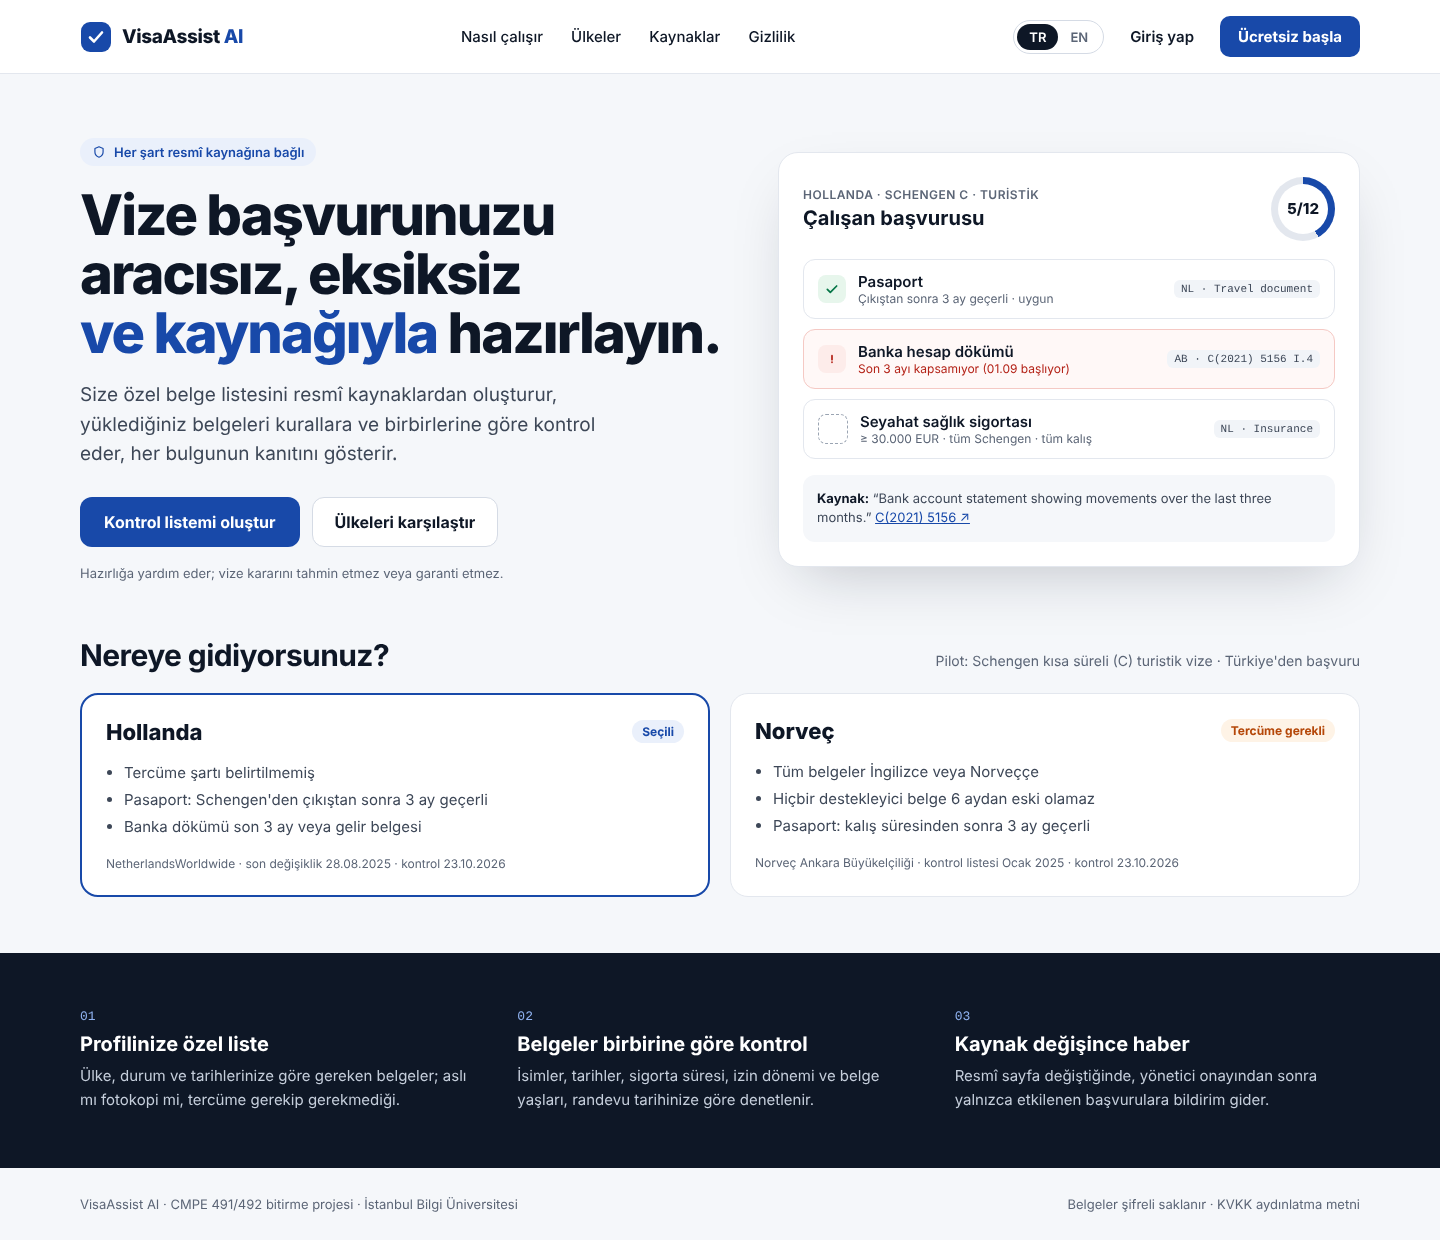
\includegraphics[width=\textwidth]{01-web-home.png}
  \caption{Home page and destination discovery.}
\end{figure}

\begin{figure}[p]
  \centering
  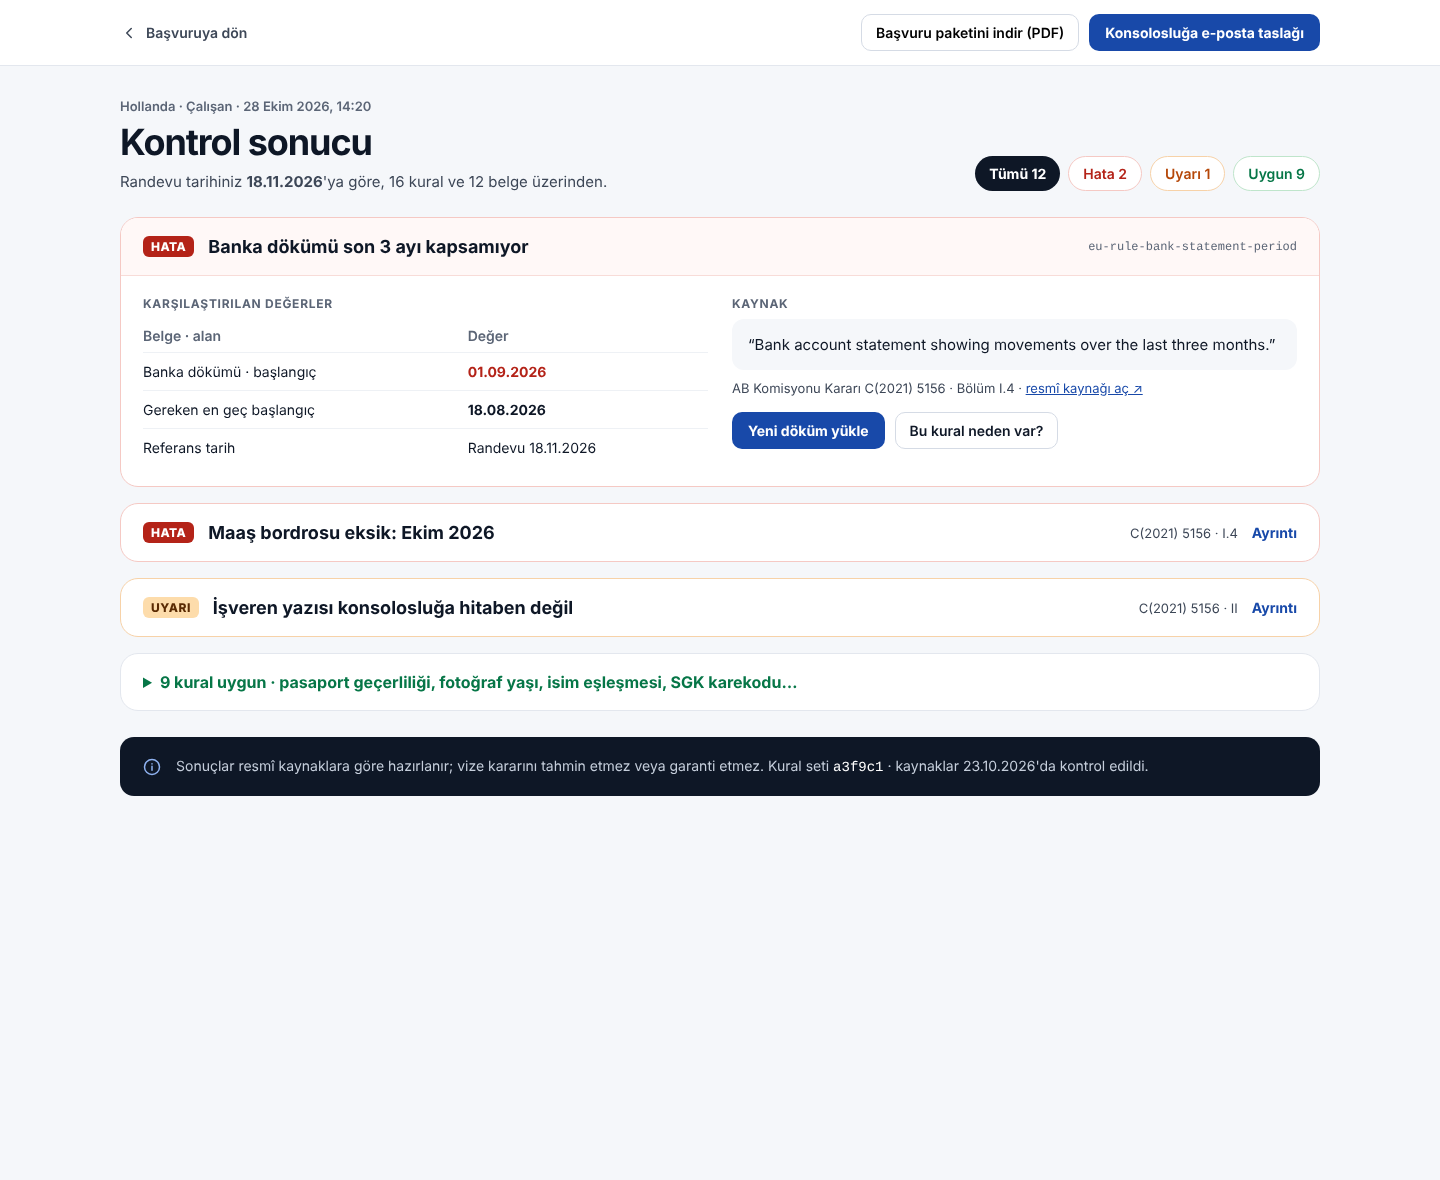
\includegraphics[width=\textwidth]{04-web-findings.png}
  \caption{Check result with compared values and the cited source passage.}
\end{figure}

\begin{figure}[ht]
  \centering
  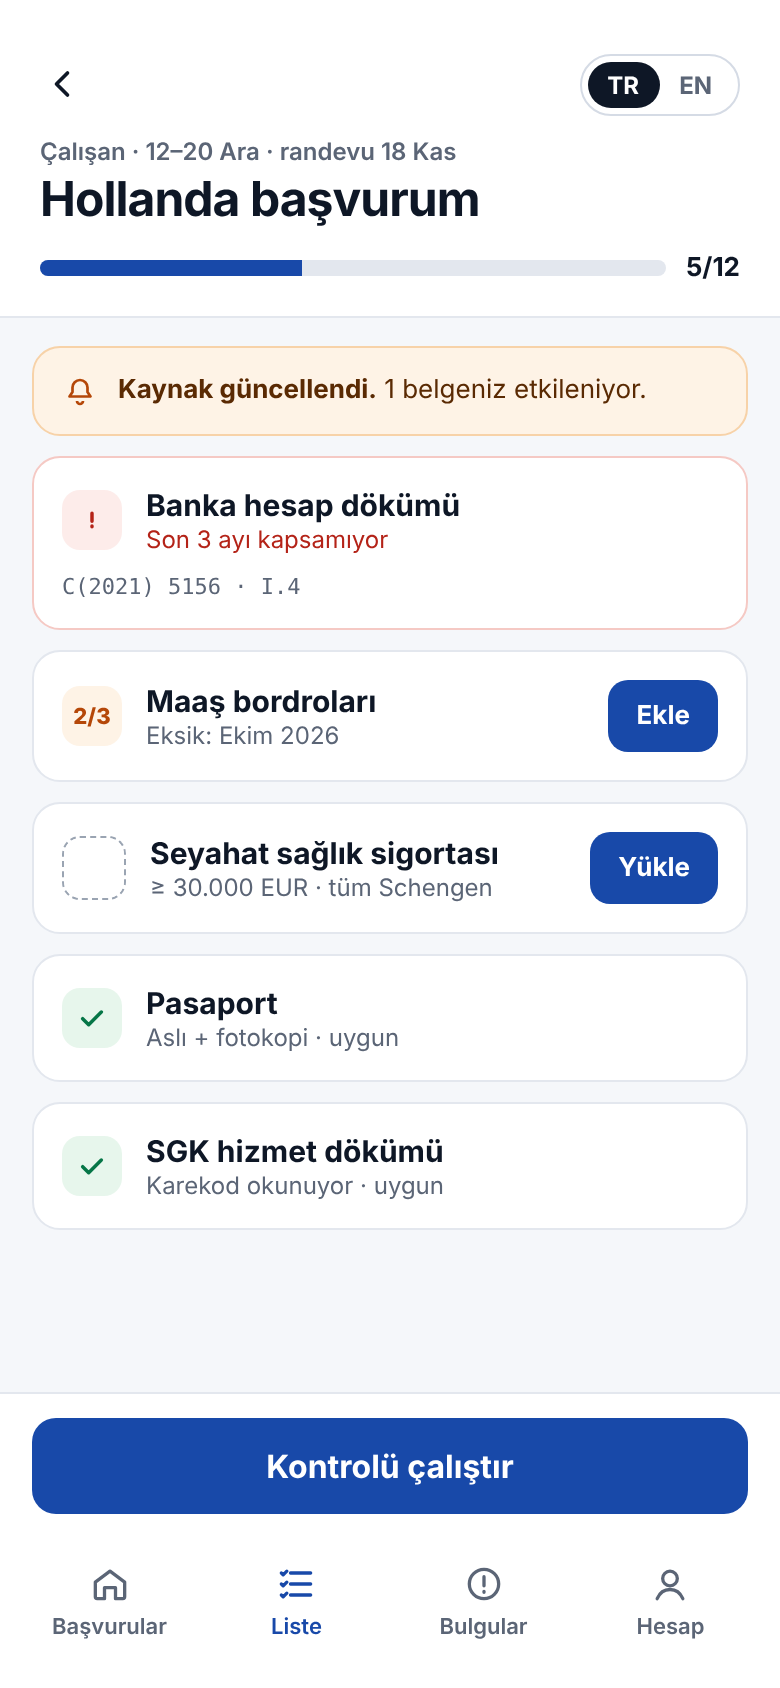
\includegraphics[width=0.31\textwidth]{06-mobile-checklist.png}\hfill
  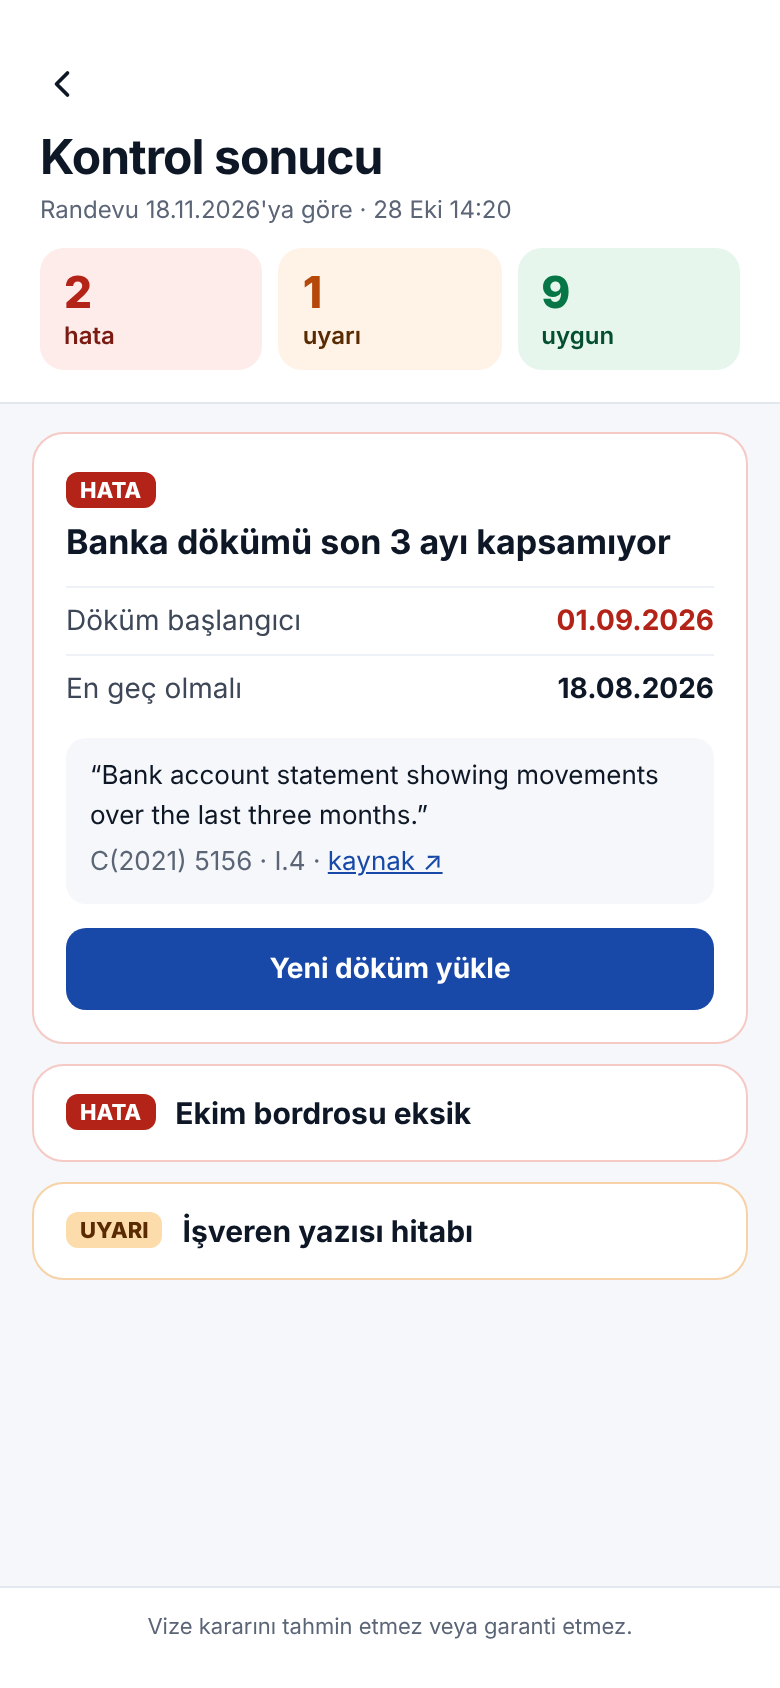
\includegraphics[width=0.31\textwidth]{08-mobile-findings.png}\hfill
  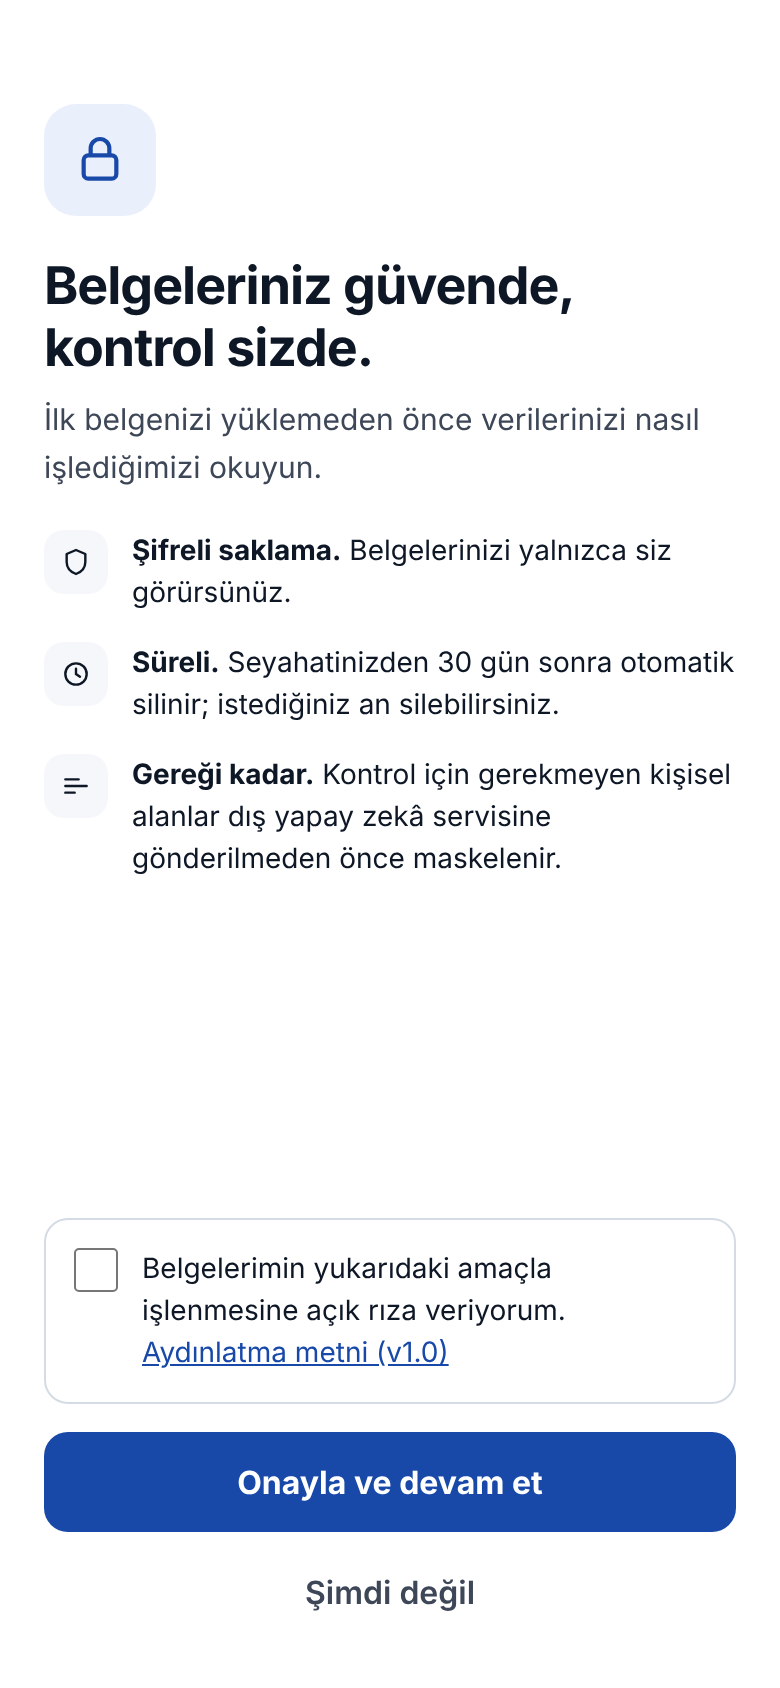
\includegraphics[width=0.31\textwidth]{09-mobile-consent.png}
  \caption{Mobile: checklist, check result and consent before the first upload.}
\end{figure}


\end{document}
